%==========================================
% Latin.Science 2026 -- Latinoware (23a edicao)
% Modalidade: SHORT PAPER (Trabalho em Andamento) -- 3 a 4 paginas
% Template oficial: IEEEtran adaptado
%==========================================

\documentclass[10pt,conference]{IEEEtran}

\usepackage[utf8]{inputenc}
\usepackage[brazil]{babel}
\usepackage{cite}

\ifCLASSINFOpdf
   \usepackage[pdftex]{graphicx}
   \graphicspath{{figs/}}
   \DeclareGraphicsExtensions{.pdf,.jpg,.jpeg,.png}
\else
   \usepackage[dvips]{graphicx}
   \graphicspath{{figs/}}
   \DeclareGraphicsExtensions{.eps}
\fi

\usepackage[cmex10]{amsmath}
\interdisplaylinepenalty=2500
\usepackage{array}
\usepackage[caption=false,font=footnotesize]{subfig}
\usepackage{url}

\hyphenation{op-tical net-works semi-conduc-tor}

% PACOTES RELACIONADOS A ADICAO DO CABECALHO DAS PAGINAS (nao alterar)
\usepackage[left=1.6cm,top=4cm,right=1.6cm,bottom=1.5cm,headheight=1cm]{geometry}
\usepackage{tikz}
\usetikzlibrary{positioning, arrows.meta, fit}
\usepackage{fancyhdr}
\usepackage{tikzpagenodes}
\renewcommand{\headrulewidth}{0pt}
\renewcommand{\footrulewidth}{0pt}
\usetikzlibrary{calc}
\pagestyle{fancy}
\setlength\headheight{10.0pt}
\addtolength{\textheight}{-40.0pt}

\fancyhead[L]{\begin{tikzpicture}[remember picture,overlay]
\draw  let \p1=($(current page.north)-(current page header area.south)$),
      \n1={veclen(\x1,\y1)} in
node [inner sep=0,outer sep=0,below right]
      at (current page.north west){
\includegraphics[width=\paperwidth,height=\n1]{headerimg.png}};
\end{tikzpicture}}

\fancyfoot[R]{\begin{tikzpicture}[remember picture,overlay]
\draw  let \p1=($(current page footer area.north)-(current page.south)$),
      \n1={veclen(\x1,\y1)} in
node [inner sep=0,outer sep=0,above right]
      at (current page.south west){
\includegraphics[width=\paperwidth,height=\n1]{footerimg.png}};
\end{tikzpicture}}

\begin{document}

\title{ARIA: Pipeline Hierárquico \textit{Teacher-Student} para\\
Detecção Automatizada de Anomalias em Rochas Ornamentais}

%-------------------------------------------------------------------------
%------------------------IMPORTANTE---------------------------------------
% CHAVE ÚNICA DE ANONIMIZAÇÃO
%   \finalfalse -> versão CEGA (submissão ao JEMS): sem autores, sem
%                  instituição, sem menção à plataforma Hartheus.
%   \finaltrue  -> versão FINAL (pós-aceite): restaura tudo automaticamente.
% Basta trocar a linha abaixo. Todo o resto do texto se ajusta sozinho via \blind.
\newif\iffinal
\finalfalse
%-------------------------------------------------------------------------
% \blind{<texto da versão CEGA>}{<texto da versão FINAL>}
\newcommand{\blind}[2]{\iffinal#2\else#1\fi}
\newcommand{\cmtid}{[preencher com o ID do JEMS]}
%-------------------------------------------------------------------------

\iffinal
% ATENÇÃO: conferir quem assina (orientador do PD1) e o e-mail antes da versão final.
\author{
\IEEEauthorblockN{Henrique Machado de Oliveira}
\IEEEauthorblockA{Instituto Federal do Espírito Santo\\
Cachoeiro de Itapemirim, Brasil\\
rikemachado999@gmail.com}
\and
\IEEEauthorblockN{[Nome do orientador]}
\IEEEauthorblockA{Instituto Federal do Espírito Santo\\
Cachoeiro de Itapemirim, Brasil\\
[e-mail]}}
\else
  \author{ID do artigo Latin.Science 2026: \cmtid \\ }
\fi

\maketitle
\thispagestyle{fancy}

\renewcommand{\abstractname}{Abstract}
\begin{abstract}
Surface quality control of ornamental stone slabs is still largely manual, subjective and hard to standardize, and the classification derived from it defines the commercial value of the slab. This paper presents ARIA, a hierarchical computer-vision pipeline in which a prior taxonomic classification restricts the visual domain of a \textit{Teacher-Student} segmenter: the Segment Anything Model (SAM), guided by lithology-calibrated textual prompts, generates annotations (\textit{pseudo-labels}) that train specialist YOLO11-seg models. The working hypothesis is that such specialization reduces false positives when compared to a single monolithic generalist model. Preliminary results on a single lithology of a real industrial dataset show that the foundation model segments relevant anomalies in a zero-shot setting when guided by calibrated prompts, supporting the feasibility of automated annotation without extensive manual labeling.
\end{abstract}

\renewcommand{\IEEEkeywordsname}{Keywords}
\begin{IEEEkeywords}
computer vision; semantic segmentation; foundation models; pseudo-labeling; ornamental stones.
\end{IEEEkeywords}

\renewcommand{\abstractname}{Resumo}
\begin{abstract}
A inspeção de anomalias superficiais em chapas de rochas ornamentais é majoritariamente manual, subjetiva e de difícil padronização, e a classificação dela derivada define o valor comercial da chapa. Este artigo apresenta o ARIA (Análise e Reconhecimento Inteligente de Anomalias), um \textit{pipeline} hierárquico de visão computacional no qual uma classificação taxonômica prévia restringe o domínio visual de um segmentador \textit{Teacher-Student}: o \textit{Segment Anything Model} (SAM), guiado por \textit{prompts} textuais calibrados por litologia, gera anotações (\textit{pseudo-labels}) que treinam modelos especialistas YOLO11-seg. A hipótese de trabalho é que essa especialização reduz falsos positivos frente a um modelo generalista monolítico. Os resultados preliminares, obtidos sobre uma única litologia de um conjunto de dados industriais reais, mostram que o modelo de fundação segmenta anomalias relevantes em regime \textit{zero-shot} quando guiado por \textit{prompts} calibrados, sustentando a viabilidade da anotação automatizada sem rotulagem manual extensiva.
\end{abstract}

\renewcommand{\IEEEkeywordsname}{Palavras-chave}
\begin{IEEEkeywords}
visão computacional; segmentação semântica; modelos de fundação; pseudo-rotulagem; rochas ornamentais.
\end{IEEEkeywords}

\IEEEpeerreviewmaketitle

\section{Introdução}

O controle de qualidade de chapas é uma etapa crítica da indústria de rochas ornamentais, setor estratégico para as exportações brasileiras e fortemente concentrado no Espírito Santo, principal polo produtor e exportador do país~\cite{stone_economy_bahiense2023}. Nessa etapa, a identificação de anomalias superficiais --- fissuras, veios, manchas e oxidações, entre outras --- determina a classificação da chapa e, por consequência, o seu valor comercial final. A tarefa é realizada de forma majoritariamente manual, dependendo da percepção visual do operador~\cite{stone_inspection_vidal2013}.

Essa inspeção carrega limitações estruturais. Não existe critério único e padronizado para definir o que constitui uma anomalia, de modo que operadores diferentes avaliam a mesma chapa de maneiras distintas. A própria experiência do avaliador atua como variável, somando-se a ela a fadiga ao longo da jornada e a natureza repetitiva da atividade. O resultado é um processo inerentemente subjetivo e de difícil padronização~\cite{stone_subjectivity_castro2018}, cuja inconsistência se traduz em precificação imprecisa e em perdas industriais.

A automação dessa inspeção por visão computacional esbarra em dois obstáculos. O primeiro é a alta variabilidade geológica das rochas: uma feição que constitui anomalia comercial em uma litologia (uma fissura em mármore branco) pode ser um padrão natural esperado em outra (um veio mineral em granito). Modelos generalistas monolíticos, treinados sobre todas as litologias simultaneamente, tendem a confundir essas feições e a gerar falsos positivos. O segundo é o custo da anotação: a rotulagem manual de milhares de imagens com defeitos sutis é onerosa e limitante para a adoção industrial.

Este trabalho apresenta o ARIA (Análise e Reconhecimento Inteligente de Anomalias), um \textit{pipeline} hierárquico\blind{}{, concebido para ser o núcleo inteligente da plataforma industrial Hartheus,} que articula três estágios: um classificador taxonômico baseado na arquitetura Xception~\cite{xception_chollet2017}, que identifica o domínio litológico da chapa; o \textit{Segment Anything Model} (SAM)~\cite{sam_kirillov2023}, que atua como Professor em uma arquitetura \textit{Teacher-Student}, gerando anotações automatizadas; e modelos YOLO11~\cite{yolo11_khanam2024}, que atuam como Alunos especialistas, otimizados para inferência rápida na linha de produção. A pergunta que orienta a investigação é: \textit{uma abordagem hierárquica --- na qual a classificação taxonômica prévia restringe o domínio visual do segmentador --- reduz os falsos positivos na detecção de anomalias superficiais, em comparação a modelos generalistas monolíticos?} A hipótese central (H1) é que modelos especialistas, por conhecerem a aparência normal de cada litologia, apresentam menor índice de falsos positivos que um modelo generalista único.

Trata-se de um \textbf{trabalho em andamento}: a contribuição aqui reportada é a calibração do modelo de fundação por litologia e a geração automatizada de anotações, cuja viabilidade se demonstra qualitativamente. A validação quantitativa de H1 depende do treinamento dos Alunos e constitui a etapa subsequente.

\begin{figure*}[!t]
  \centering
  \resizebox{0.80\textwidth}{!}{%
  \begin{tikzpicture}[
    node distance=0.5cm and 0.7cm,
    box/.style={draw, rounded corners, align=center, minimum height=1.1cm,
      text width=2.9cm, font=\small, inner sep=4pt},
    io/.style={draw, align=center, font=\small, text width=2.0cm, inner sep=4pt},
    arr/.style={-{Latex[length=2.2mm]}, thick}
  ]
    \node[io] (in) {Imagem da chapa};
    \node[box, right=of in] (xc) {\textbf{Xception}\\classifica o tipo litológico};
    \node[box, right=of xc] (sam) {\textbf{SAM3} (Professor)\\anotações calibradas por litologia};
    \node[box, right=of sam] (yolo) {\textbf{YOLO11-seg} (Aluno) $\times\,45$\\inferência rápida};
    \node[io, right=of yolo] (out) {Polígonos de anomalias};
    \draw[arr] (in) -- (xc);
    \draw[arr] (xc) -- (sam);
    \draw[arr] (sam) -- (yolo);
    \draw[arr] (yolo) -- (out);
    \node[draw, dashed, fit=(sam)(yolo), inner sep=8pt,
      label={[font=\small\itshape]above:Teacher--Student}] {};
  \end{tikzpicture}%
  }
  \caption{\textit{Pipeline} hierárquico do ARIA: a classificação taxonômica restringe o domínio visual do segmentador especialista \textit{Teacher-Student}, no qual o SAM gera as anotações que treinam os modelos YOLO11.}
  \label{fig:arquitetura}
\end{figure*}

\section{Trabalhos Relacionados}

A inspeção visual automatizada (\textit{Automated Visual Inspection} --- AVI) para detecção de defeitos é tema consolidado em setores como têxtil~\cite{avi_textile_sikka2024} e construção civil~\cite{avi_concrete_waqar2024}. Levantamentos recentes sobre detecção de anomalias visuais industriais evidenciam um gargalo recorrente: a maioria das abordagens depende de aprendizado supervisionado e, portanto, de grandes volumes de imagens anotadas manualmente~\cite{avi_anomaly_li2025}. Esse custo é particularmente limitante em domínios de alta variabilidade visual, em que cada litologia exige exemplos próprios.

No contexto específico das rochas ornamentais, os trabalhos existentes concentram-se na \textit{classificação} do tipo de rocha, e não na \textit{segmentação} de anomalias superficiais. Técnicas de aprendizado de máquina já foram aplicadas à classificação de pedras ornamentais~\cite{stone_lopez2010} e redes convolucionais profundas à tipificação automatizada de rochas~\cite{rocktyping_baraboshkin2020}; na classificação de chapas polidas, destacam-se um estudo inicial com redes convolucionais~\cite{deepstone_araujo2022} e o DeepStoneAI~\cite{deepstoneai_moreira2025}\blind{}{, ambos desenvolvidos no mesmo campus desta pesquisa}, que compara quatro arquiteturas sobre 45 litologias comerciais. Identifica-se, assim, uma lacuna: a detecção de anomalias superficiais em rochas ornamentais permanece pouco explorada, enquanto as abordagens de AVI disponíveis esbarram no custo da anotação manual.

Para contorná-lo, este trabalho recorre a duas linhas consolidadas. A primeira é a dos Modelos de Fundação, representada pelo SAM~\cite{sam_kirillov2023}, guiado por engenharia de \textit{prompts}. A segunda é a da transferência de conhecimento por arquitetura \textit{Teacher-Student}~\cite{distill_hinton2015} acoplada a \textit{pseudo-labeling}~\cite{pseudolabel_lee2013}: um modelo robusto e computacionalmente caro processa as imagens \textit{offline} e supervisiona o treinamento de um modelo menor, otimizado para inferência. Como Aluno, adota-se o YOLO11~\cite{yolo11_khanam2024}, que executa extração de características e predição de máscaras em uma única passagem, viabilizando a inferência em tempo real na linha de produção.

\section{Materiais e Métodos}

A Figura~\ref{fig:arquitetura} resume o \textit{pipeline}. O diferencial da proposta está em usar a classificação litológica como \textbf{restrição de domínio}: em vez de um segmentador único para todas as rochas, cada litologia recebe uma configuração própria de \textit{prompts} e limiares e, ao final, um modelo Aluno próprio.

\subsection{Conjunto de Dados}

O conjunto reúne 34.630 imagens industriais reais de chapas~\cite{dataset_araujo2023}, distribuídas em 45 litologias e preservando o desbalanceamento natural da produção --- algumas variedades contam com poucas amostras, o que exigirá curadoria e, possivelmente, o agrupamento das mais raras. As anomalias consideradas na calibração são fissuras (\textit{crack}), veios minerais (\textit{vein}), manchas (\textit{stain}), áreas escuras ou oxidações em rochas claras (\textit{dark patches}) e pontos claros em rochas escuras (\textit{light spot}). Vale notar que o mesmo padrão visual pode constituir defeito em uma litologia e característica estética em outra --- o que reforça a necessidade de restringir o domínio antes de segmentar.

\subsection{Calibração do Professor por Litologia}

A injeção de conhecimento de domínio no Professor é operacionalizada por um arquivo de configuração que associa, a cada litologia, um conjunto de \textit{prompts} de anomalia e um limiar próprio para cada um deles --- o grau de confiança com que o modelo julga que a região segmentada corresponde ao \textit{prompt}. A motivação é direta: um limiar adequado para realçar fissuras em um mármore branco tende a super-segmentar a textura de um granito escuro, produzindo falsos positivos.

Adota-se o SAM3, variante do SAM com suporte a \textit{prompts} textuais abertos, cuja interpretação se apoia no CLIP~\cite{clip_radford2021} --- que projeta texto e imagem em um espaço de \textit{embeddings} compartilhado, aproximando o vetor de uma palavra das regiões visualmente similares. Como o CLIP foi treinado a partir de legendas, e não de palavras isoladas, \textit{prompts} contextuais (por exemplo, \textit{crack on a stone surface}) tendem a desambiguar melhor o alvo do que termos isolados, que podem evocar contextos alheios ao domínio. Em vez de ajustar 45 configurações independentes a partir do zero, as litologias foram organizadas em grupos por cor e textura, que compartilham estratégias de \textit{prompt} e faixas de limiar semelhantes, com refinamentos individuais quando necessário (Tabela~\ref{tab:calibracao}). A configuração padrão de referência adota limiares de 0,1 para \textit{crack}, 0,007 para \textit{vein} e 0,3 para \textit{stain}.

\begin{table}[!t]
\renewcommand{\arraystretch}{1.2}
\caption{Estratégias de Calibração de \textit{Prompts} e Limiares por Grupo de Litologia}
\label{tab:calibracao}
\centering
\footnotesize
\begin{tabular}{|l|p{5.0cm}|}
\hline
\textbf{Grupo} & \textbf{Ajuste característico} \\
\hline
Brancas / claras & Incluem \textit{dark patches}; limiares próximos do padrão \\
\hline
Escuras & Usam \textit{light spot} no lugar de \textit{dark patches}; limiares mais baixos (ex.: 0,05 e 0,01) \\
\hline
Amarelas / bege & Incluem \textit{dark patches}; limiares intermediários entre claras e escuras \\
\hline
Verdes / quartzitos & Sem \textit{dark patches}; \textit{crack} entre 0,06 e 0,08 \\
\hline
Coloridas (vermelhas) & Incluem \textit{light spot}; \textit{crack} em 0,07 \\
\hline
Especiais & Configurações individuais, próximas do padrão \\
\hline
\end{tabular}
\end{table}

A imagem representativa de cada litologia é escolhida \textbf{manualmente} --- empregar o próprio SAM para selecioná-la configuraria raciocínio circular. Sobre ela, ajusta-se a configuração de forma iterativa até que as máscaras sejam consideradas satisfatórias, e as anotações finais são exportadas como polígonos no formato de segmentação do YOLO. Nesta versão, todas as anomalias são tratadas como uma única classe genérica, pois a distinção semântica entre tipos depende da qualidade dos \textit{embeddings} de texto, ainda não validada de forma independente.

\subsection{Protocolo Experimental e de Avaliação}

O experimento central avalia H1 comparando dois \textit{pipelines} treinados sobre a mesma arquitetura YOLO11-seg. No especialista (ARIA), o classificador identifica o tipo litológico e seleciona os \textit{prompts} calibrados correspondentes, resultando em \textbf{45 modelos}, cada um treinado exclusivamente nas anotações de sua litologia. No \textit{baseline} generalista, o estágio de classificação é ausente: o SAM3 usa uma configuração genérica e um \textbf{único modelo} YOLO é treinado com as anotações de todos os tipos. A comparação confronta, portanto, os dois \textit{pipelines} completos; separar o efeito da anotação calibrada do efeito da especialização exigiria um braço intermediário --- SAM3 calibrado com modelo único ---, previsto como extensão.

Avaliar cada Aluno contra os pseudo-rótulos que o treinaram seria circular: cada braço venceria no gabarito produzido por seu próprio Professor. Ambos são, por isso, avaliados sobre um \textbf{conjunto de teste comum} --- amostra estratificada por litologia, anotada manualmente por professores especializados no setor de rochas ornamentais e externa aos pseudo-rótulos dos dois braços ---, com divisão de 70/20/10 entre treino, validação e teste. Reportam-se a Interseção sobre União (IoU) e a precisão média (mAP)~\cite{voc_everingham2010} e, por vincular-se diretamente a H1, a precisão e a taxa de falsos positivos por imagem, além do tempo de inferência de Professor e Aluno. A análise quantitativa é complementada pela inspeção qualitativa das máscaras pelos mesmos especialistas. O desenvolvimento utiliza Python com PyTorch e processamento paralelo em GPU.\blind{ O código e os arquivos de configuração serão disponibilizados publicamente.}{ O código e os arquivos de configuração estão disponíveis em \url{https://github.com/machado-o/ARIA}.}

\section{Resultados e Discussão}

\subsection{Classificação Litológica}

O estágio de classificação taxonômica reaproveita o DeepStoneAI~\cite{deepstoneai_moreira2025}; os números a seguir são reportados por aquele trabalho, avaliado sobre as 45 litologias deste mesmo conjunto de dados, e reproduzidos aqui apenas para contextualizar o primeiro estágio. Entre quatro arquiteturas comparadas, a Xception obteve a maior acurácia (99,21\%), com a maior parte dos tipos perfeitamente classificada e confusão residual concentrada em duas variedades visualmente semelhantes. O desempenho sustenta um roteamento confiável, mas convém registrar que o roteamento incorreto é um modo de falha próprio da hierarquia --- ausente no \textit{baseline} monolítico --- que a avaliação de ponta a ponta precisa contabilizar.

\subsection{Geração de Anotações pelo Professor}

Os resultados a seguir foram obtidos na litologia \textit{ice leke}, primeira a ter \textit{prompts} e limiares plenamente ajustados e adotada como caso de demonstração por exibir anomalias visualmente nítidas. A partir de uma imagem industrial real, o SAM3 foi guiado pelos \textit{prompts} calibrados e segmentou as anomalias superficiais \textbf{sem qualquer treinamento prévio específico para rochas ornamentais}. A Figura~\ref{fig:resultado} contrapõe a imagem original às máscaras sobrepostas, geradas de forma totalmente automatizada. A inspeção das máscaras isoladas por \textit{prompt} sugere que cada descrição textual atua sobre um tipo distinto de irregularidade --- fissuras, veios, manchas e áreas escuras ---, sem que essa separação tenha sido validada quantitativamente; daí a opção pela rotulagem binária.

\begin{figure}[!t]
  \centering
  \subfloat[Imagem original da chapa]{%
    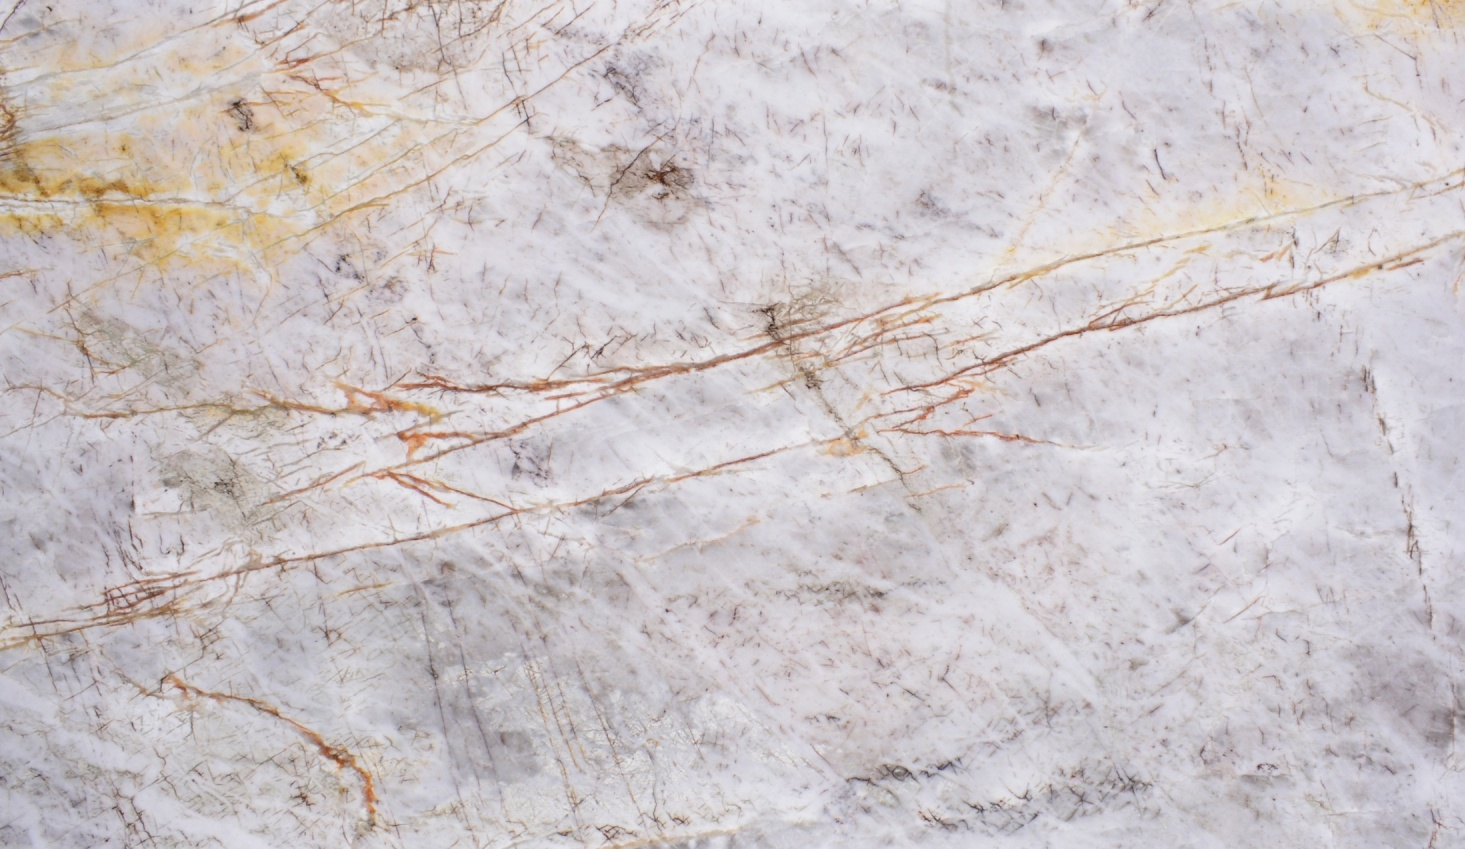
\includegraphics[width=0.47\columnwidth]{figs/sample_ice_leke_original.jpg}}
  \hfil
  \subfloat[Anotações geradas pelo SAM]{%
    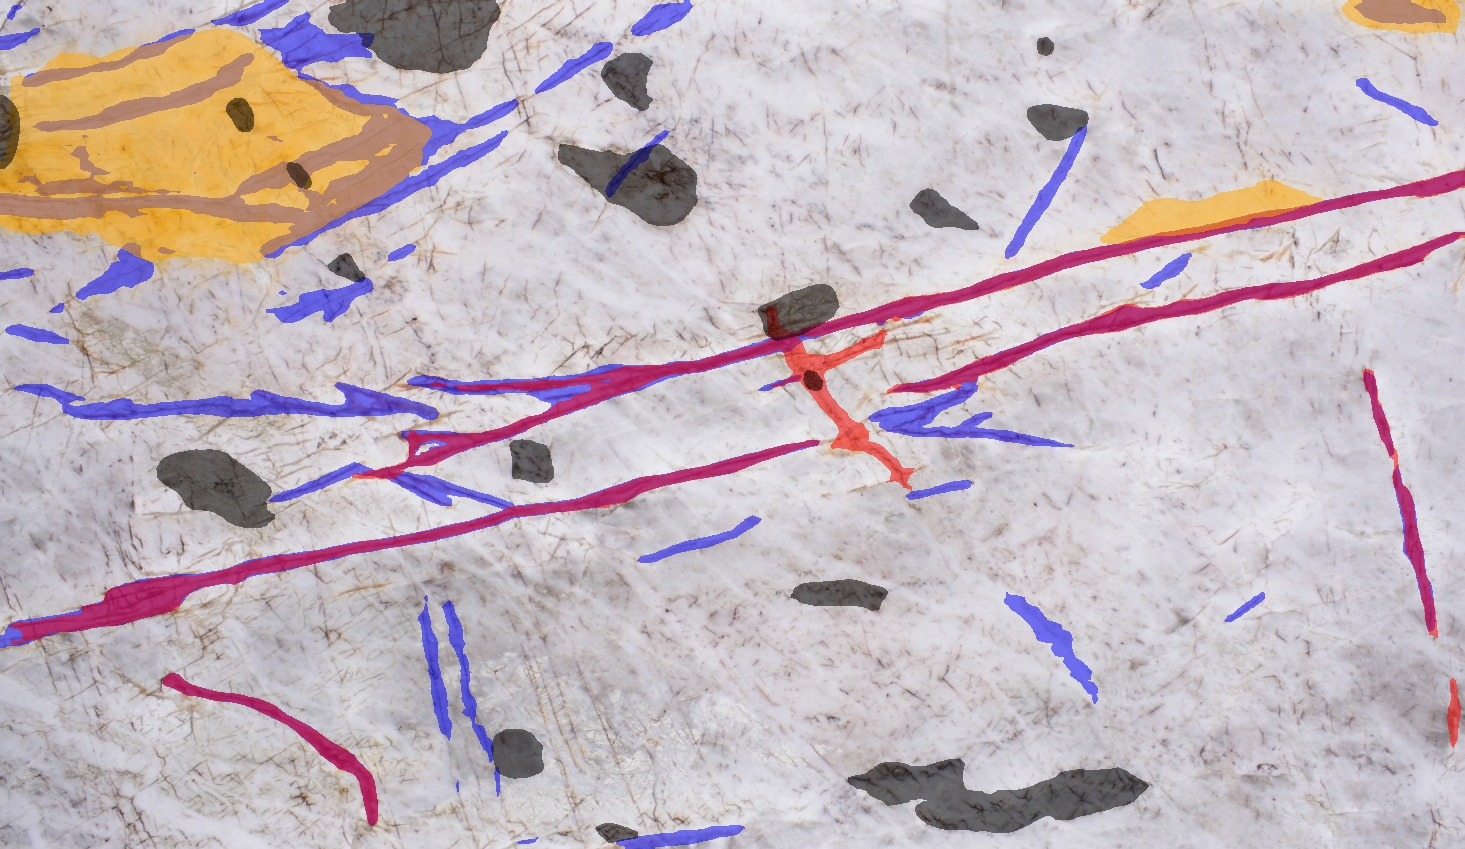
\includegraphics[width=0.47\columnwidth]{figs/sample_ice_leke_combined.jpg}}
  \caption{Segmentação automatizada de anomalias na litologia \textit{ice leke}: imagem original (a) e máscaras sobrepostas geradas em regime \textit{zero-shot} (b).}
  \label{fig:resultado}
\end{figure}

\subsection{Discussão e Limitações}

Os resultados confirmam a viabilidade da etapa central: um modelo de fundação, sem treinamento dedicado ao domínio, segmenta anomalias relevantes quando guiado por \textit{prompts} calibrados por litologia, e a cadeia de anotação automatizada está operacional de ponta a ponta.

As limitações são explícitas. A validação é \textbf{qualitativa e preliminar}: das 45 litologias, apenas a primeira está plenamente calibrada. Não há ainda medida quantitativa da qualidade das anotações, e a evidência reportada sustenta a \textit{viabilidade} da geração automatizada, mas \textbf{não testa H1} --- a comparação entre os \textit{pipelines} depende do treinamento dos modelos Alunos. Persiste também o risco, inerente ao \textit{pseudo-labeling}, de que erros sistemáticos do Professor sejam herdados pelo Aluno, o que motiva a validação por especialistas prevista no protocolo.

\section{Conclusões}

Este artigo apresentou o ARIA, um \textit{pipeline} hierárquico \textit{Teacher-Student} para detecção automatizada de anomalias em chapas de rochas ornamentais, e suas evidências preliminares. A classificação taxonômica prévia mostra-se confiável o bastante para rotear as chapas, e a calibração de \textit{prompts} e limiares por litologia permite que um modelo de fundação gere anotações poligonais úteis em regime \textit{zero-shot}, atacando diretamente o gargalo do custo de anotação.

Os próximos passos são concluir a calibração das 45 litologias, treinar os modelos especialistas e o \textit{baseline} generalista e realizar a comparação quantitativa que testa a hipótese central. Como trabalhos futuros registram-se ainda o \textit{loop} de aprendizado ativo, com o Professor refinando predições de baixa confiança do Aluno em produção, e a rotulagem multiclasse por tipo de anomalia, que requer validação humana de uma amostra das anotações.

\section*{Agradecimentos}

\blind{\textit{Omitidos para revisão cega.}}{Os autores agradecem ao Instituto Federal do Espírito Santo --- Campus Cachoeiro de Itapemirim e às empresas do setor de rochas ornamentais que viabilizaram o acesso às imagens industriais utilizadas neste trabalho.}

\section*{Declaração sobre uso de Inteligência Artificial}

Declaro que ferramentas de Inteligência Artificial Generativa foram utilizadas neste trabalho nas seguintes etapas: o assistente Claude (Anthropic) apoiou a redação e a revisão crítica do texto, na etapa de escrita, e a implementação dos \textit{scripts} de calibração e inferência, na etapa de desenvolvimento. Nenhum dado, experimento ou resultado foi gerado por IA. Todo o conteúdo gerado foi revisado criticamente e validado pelo autor, que assume integral responsabilidade pela originalidade e veracidade do texto final, em conformidade com a Portaria CNPq n° 2.664/2026.

\bibliographystyle{IEEEtran}
\bibliography{referencias}

\end{document}
